\documentclass[]{article}

% Imported Packages
%------------------------------------------------------------------------------
\usepackage{amssymb}
\usepackage{amstext}
\usepackage{amsthm}
\usepackage{amsmath}
\usepackage{enumerate}
\usepackage{fancyhdr}
\usepackage[margin=1in]{geometry}
\usepackage{graphicx}
\usepackage{extarrows}
\usepackage{setspace}
\usepackage{float}
\usepackage{verbatim}
%------------------------------------------------------------------------------

% Header and Footer
%------------------------------------------------------------------------------
\pagestyle{plain}  
\renewcommand\headrulewidth{0.4pt}                                      
\renewcommand\footrulewidth{0.4pt}                                    
%------------------------------------------------------------------------------

% Title Details
%------------------------------------------------------------------------------
\title{Deliverable \#2 Tutorial 2 Group 5}
\author{SE 3A04: Software Design II -- Large System Design}
\date{}                               
%------------------------------------------------------------------------------

% Document
%------------------------------------------------------------------------------
\begin{document}

\maketitle	

\section{Introduction}
\label{sec:introduction}

The following document is a description of the desired interaction between the intended user and the systems, as well as the architectural details of the software. 

\subsection{Purpose}
\label{sub:purpose}
The purpose of this document is twofold. First, it is to provide a higher-level view of the system, using simplified graphical representation of what the system must do. Second, it is to provide a basic general guideline for architectural implementation of the systems within the software. The intended audience of this document is mainly focused for the developers of the software by generalizing the internal details of the software, however any stakeholders may find the document of interest as the functional requirements are conveyed here.

\subsection{System Description}
\label{sub:system_description}
SpaceBase Ephemeris (SBE) is a real-time system that simulates a human settlement on a foreign planet, named Ephemeris.  The simulation takes place in a distant future where technology has improved to sustain humankind on extraterrestrial planets which are otherwise uninhabitable. As a commander of the base, the user has the responsibility of manipulating the sub-systems to ensure all of the key operations are functional, and possibly ideal. The three subsystems are power control, atmospheric simulation, and the station personnel.

\subsection{Overview}
\label{sub:overview}
The first part of this document provides a graphical representation of the functional requirements of the software and how it must interact with the intended users using an use case diagram. The remainder of the document provides guidelines for internal design of the software, using an analysis class diagram, a detailed discussion on the architectural design of the system, and a series of class responsibility collaboration cards. 


\section{Use Case Diagram}
\label{sec:use_case_diagram}
\begin{figure}[H]
	\centering
	\includegraphics[width=100mm]{3A04-Deliverable2-usecase.png}
	\caption{The use case diagram}
\end{figure}
\begin{enumerate}
	\item Create New Station: The users opens the application to the main menu. They select the new-station button. They enter parameters for the station such as size, or accept the defaults, then confirm. The game generates a station with the selected parameters, initializes the subsystems, then opens and displays the new station.
	\item Load: The user opens the application to the main menu. They select the load-previous-save button, then selects the appropriate file on their device. The game deserializes the game-state from the file, initializes the subsystems, then opens it and displays it.
	\item Save: The user pauses while playing the game, then selects the save-game button. They enter an appropriate filename into the prompt given. The system serializes the game-state, and writes it to the file location given, then returns to the pause screen.
	\item Change Setting: The user pauses while playing the game, then selects the settings button. The user enters a new value for one of the settings displayed (for example changing the speed at which personnel move and act). The user confirms the new setting, causing the subsystems to implement it, and react appropriately to any changes in the world it may cause.
	\item Issue Order: The user selects a location within the station. They select that a generator should be built at that location. The personnel subsystem determines which personnel will carry out the order, and assigns them to do so. As time passes, the assigned personnel install the generator.
	\item Operate Device: The user selects an airlock door in the station to be opened. The power subsystem then checks that the door is powered, and operates it. The atmospheric subsystem circulates gases between the two sides to correct any imbalances. The personnel system reroutes personnel through the door if it creates a shorter path to their destination.
	\item Check Views: The users pauses while playing the game. They toggle on or off any number of subsystem views, then return to gameplay. The game now displays the selected views.
	\item Snapshot: The user pauses while playing the game. They select the snapshot button and are prompted to enter their user credentials for Twitter. They enter them and confirm. If the system determines the credentials are valid, it creates a picture out of the current game state and views, then posts the picture with the user's credentials, and returns the user to the game.
\end{enumerate}


\section{Analysis Class Diagram}
\label{sec:analysis_class_diagram}
\begin{figure}[H]
	\centering
	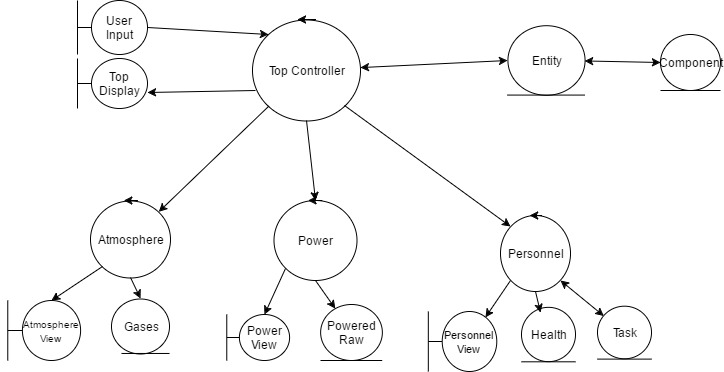
\includegraphics[width=120mm]{ACD_primitives.jpg}
	\caption{The analysis class diagram}
\end{figure}


\section{Architectural Design}
\label{sec:architectural_design}
This section should provide an overview of the overall architectural design of your application. You overall architecture should show the division of the system into subsystems with high cohesion and low coupling.

\subsection{System Architecture}
\label{sub:system_architecture}
The overall architecture of the system is a \textbf{Presentation, Abstraction, and Control (PAC)} architecture. The three subsystems, as well as a few other major components are all PAC agents, with a single master PAC agent which orchestrates them. The PAC architecture was chosen first because it is an effective architecture for interaction-orientated software. It was chosen over other such architectures because it is an effective model for systems with a set of agents, each with their own model and interface, such as this. It is useful for situations where agents may need to be easily removed, replaced, or added later in development, a requirement for this system. Since each subsystem must have a separate, toggle-able view, an architecture that supports multiple Presentations is a good choice. The hierarchical nature of PAC allows for low coupling as subsystems can have an overarching controller which can orchestrate communication, rather than tying each subsystem directly to each other subsystem. Lastly, MVC is a poor choice as it would lead to low cohesion when all the subsystems are grouped into a single controller.

There is also an Entity Component System (ECS) architecture, which is common in games to simplify inheritance hierarchies and reduce coupling in cases where objects may have relevant properties to multiple subsystems (for eg, a tile may have properties relevant to both atmospheric and power subsystems). The contents of the station, such as tiles, people, and devices, are entities, which contain a set of components, each relevant to a specific subsystem.

\subsection{Subsystems}
\label{sub:subsystems}
The following is a description of the subsystems included in the system.
\begin{enumerate}[a)]
	\item Atmospheric: Simulates the flow of various gases through the station, and their effects. Various devices powered by the Power subsystem can affect these flows, and the gases (or lack thereof) can affect the Personnel subsystem by damaging the personnel.
	\item Power: Simulates the power flow through station wires, the draw of various devices, and the output of station generators. These devices can affect the Atmospheric subsystem by moving, adding, or removing gases in the station. The Power subsystem can affect the Personnel subsystem with these devices, for example a depowered airlock cannot be opened, preventing the passage of personnel.
	\item Personnel: Simulates the personnel aboard the station, and controls their movements and actions. The station personnel can directly affect the Atmospheric subsystem by slowly changing the gas composition by breathing. They can directly affect the Power subsystem by installing, removing, or using various devices in the station.
\end{enumerate}

\section{Class Responsibility Collaboration (CRC) Cards}
\label{sec:class_responsibility_collaboration_crc_cards}
This section should contain all of your CRC cards.

\begin{enumerate}[a)]
	\item Provide a CRC Card for each identified class
	\item Please use the format outlined in tutorial, i.e., 
	\begin{table}[ht]
		\centering
		\begin{tabular}{|p{5cm}|p{5cm}|}
		\hline 
		 \multicolumn{2}{|l|}{\textbf{Class Name: MainMenuGUI}} \\
		\hline
		\textbf{Responsibility:} & \textbf{Collaborators:} \\
		\hline
		Display buttons for user input & \\
		\hline
		Direct view from main menu to a new station & StationGenerator\\
		\hline
		Show user saved games upon load game request & MainMenuAbstract \\
		\hline
		Open chosen game from saved games list  & StationGenerator \\
		\hline
		On user request for settings, open settings menu & SettingsGUI\\
		\hline
		\end{tabular}
	\end{table}
	\begin{table}[ht]
		\centering
		\begin{tabular}{|p{5cm}|p{5cm}|}
		\hline 
		 \multicolumn{2}{|l|}{\textbf{Class Name: MainMenuController}} \\
		\hline
		\textbf{Responsibility:} & \textbf{Collaborators:} \\
		\hline
		Create new station & StationGenerator\\
		\hline
		Load values from saved game file into game to allow game to continue from saved state & StationGenerator\\
		\hline
		\end{tabular}
	\end{table}
	\begin{table}[ht]
		\centering
		\begin{tabular}{|p{5cm}|p{5cm}|}
		\hline 
		 \multicolumn{2}{|l|}{\textbf{Class Name: MainMenuAbstract}} \\
		\hline
		\textbf{Responsibility:} & \textbf{Collaborators:} \\
		\hline
		Store saved games and list on request & MainMenuGUI\\
		\hline
		Load values from saved game file to continue game & MainMenuController\\
		\hline
		\end{tabular}
	\end{table}
	\begin{table}[ht]
		\centering
		\begin{tabular}{|p{5cm}|p{5cm}|}
		\hline 
		 \multicolumn{2}{|l|}{\textbf{Class Name: SettingsGUI}} \\
		\hline
		\textbf{Responsibility:} & \textbf{Collaborators:} \\
		\hline
		Display settings window & \\
		\hline
		Get current settings attributes & SettingsAbstract \\
		\hline
		Display text for settings description and current settings attribute & \\
		\hline
		Display the buttons for user input & \\
		\hline
		Send new settings to abstract & SettingsController \\
		\hline
		\end{tabular}
	\end{table}
	\begin{table}[ht]
		\centering
		\begin{tabular}{|p{5cm}|p{5cm}|}
		\hline 
		 \multicolumn{2}{|l|}{\textbf{Class Name: SettingsController}} \\
		\hline
		\textbf{Responsibility:} & \textbf{Collaborators:} \\
		\hline
		Get updated settings values & SettingsGUI\\
		\hline
		Apply the new changes & SettingsAbstract\\
		\hline
		\end{tabular}
	\end{table}
	\begin{table}[ht]
		\centering
		\begin{tabular}{|p{5cm}|p{5cm}|}
		\hline 
		 \multicolumn{2}{|l|}{\textbf{Class Name: SettingsAbstract}} \\
		\hline
		\textbf{Responsibility:} & \textbf{Collaborators:} \\
		\hline
		Store settings values & \\
		\hline
		Return requested attributes & SettingsGUI\\
		\hline
		Change requested attributes & SettingsController\\
		\hline
		\end{tabular}
	\end{table}
	\begin{table}[ht]
		\centering
		\begin{tabular}{|p{5cm}|p{5cm}|}
		\hline 
		 \multicolumn{2}{|l|}{\textbf{Class Name: StationGenerator}} \\
		\hline
		\textbf{Responsibility:} & \textbf{Collaborators:} \\
		\hline
		Load default station values to create station base & \\
		\hline
		Load existing station values from file chosen in main menu and recreate station & MainMenuController\\
		\hline
		\end{tabular}
	\end{table}
	\begin{table}[ht]
		\centering
		\begin{tabular}{|p{5cm}|p{5cm}|}
		\hline 
		 \multicolumn{2}{|l|}{\textbf{Class Name:}PersonnelController} \\
		\hline
		\textbf{Responsibility:} & \textbf{Collaborators:} \\
		\hline
		Accept orders from user & TopController \\
		\hline
		Instruct personnel how to perform orders & Task \\
		\hline
		Keep personnel away from dangers & Health \\
		\hline
		Simulate personnel's condition in the presence of danger & Health \\
		\hline
		\end{tabular}
	\end{table}
	\begin{table}[ht]
		\centering
		\begin{tabular}{|p{5cm}|p{5cm}|}
		\hline 
		 \multicolumn{2}{|l|}{\textbf{Class Name:}PersonnelView} \\
		\hline
		\textbf{Responsibility:} & \textbf{Collaborators:} \\
		\hline
		Display locations of personnel &  \\
		\hline
		Display tasks of personnel &  \\
		\hline
		\end{tabular}
	\end{table}
	\begin{table}[ht]
		\centering
		\begin{tabular}{|p{5cm}|p{5cm}|}
		\hline 
		 \multicolumn{2}{|l|}{\textbf{Class Name:}Task} \\
		\hline
		\textbf{Responsibility:} & \textbf{Collaborators:} \\
		\hline 
		Store current task of a person & Component \\
		\hline
		\end{tabular}	
	\end{table}
	\begin{table}[ht]
		\centering
		\begin{tabular}{|p{5cm}|p{5cm}|}
		\hline 
		 \multicolumn{2}{|l|}{\textbf{Class Name:}Health} \\
		\hline
		\textbf{Responsibility:} & \textbf{Collaborators:} \\
		\hline 
		Store current liveliness status of a person & Component \\
		\hline
		\end{tabular}	
	\end{table}
	\begin{table}[ht]
		\centering
		\begin{tabular}{|p{5cm}|p{5cm}|}
		\hline 
		 \multicolumn{2}{|l|}{\textbf{Class Name:}PowerController} \\
		\hline
		\textbf{Responsibility:} & \textbf{Collaborators:} \\
		\hline 
		Simulate powerflow through the station & PowerDraw \\
		\hline
		Operate powered devices & Powerdraw, Device \\
		\hline
		\end{tabular}	
	\end{table}
	\begin{table}[ht]
		\centering
		\begin{tabular}{|p{5cm}|p{5cm}|}
		\hline 
		 \multicolumn{2}{|l|}{\textbf{Class Name:}PowerView} \\
		\hline
		\textbf{Responsibility:} & \textbf{Collaborators:} \\
		\hline 
		Display flow of power through the station &  PowerController\\
		\hline
		Display overall power status of station &  PowerController\\
		\hline
		\end{tabular}
	\end{table}
	\begin{table}[ht]
		\centering
		\begin{tabular}{|p{5cm}|p{5cm}|}
		\hline 
		 \multicolumn{2}{|l|}{\textbf{Class Name:}PowerDraw} \\
		\hline
		\textbf{Responsibility:} & \textbf{Collaborators:} \\
		\hline 
		Store the amount of power an entity adds or draw from the grid & Component\\
		\hline
		\end{tabular}
	\end{table}
	\begin{table}[ht]
		\centering
		\begin{tabular}{|p{5cm}|p{5cm}|}
		\hline 
		 \multicolumn{2}{|l|}{\textbf{Class Name:}PowerDraw} \\
		\hline
		\textbf{Responsibility:} & \textbf{Collaborators:} \\
		\hline 
		Store the amount of power an entity adds or draw from the grid & Component\\
		\hline
		\end{tabular}
	\end{table}
\end{enumerate}


\appendix
\section{Division of Labour}
\label{sec:division_of_labour}
\begin{enumerate}
	\item Ian: Designed use case diagram, wrote subsystem descriptions, use case scenarios, and architecture description, wrote CRC cards, designed analysis class diagram
	\item Nishanth: Designed use case diagram, designed analysis class diagram
	\item Arfa: Designed use case diagram, designed analysis class diagram
	\item Steven: Wrote Introduction section, wrote CRC cards
	\item Areeb: Drew use case diagram from the paper reference, designed use case diagram, wrote CRC cards
\end{enumerate}

\begin{comment}
\newpage
\section*{IMPORTANT NOTES}
\begin{itemize}
%	\item You do \underline{NOT} need to provide a text explanation of each diagram; the diagram should speak for itself
	\item Please document any non-standard notations that you may have used
	\begin{itemize}
		\item \emph{Rule of Thumb}: if you feel there is any doubt surrounding the meaning of your notations, document them
	\end{itemize}
	\item Some diagrams may be difficult to fit into one page
	\begin{itemize}
		\item It is OK if the text is small but please ensure that it is readable when printed
		\item If you need to break a diagram onto multiple pages, please adopt a system of doing so and thoroughly explain how it can be reconnected from one page to the next; if you are unsure about this, please ask about it
	\end{itemize}
	\item Please submit the latest version of Deliverable 1 with Deliverable 2
	\begin{itemize}
		\item It does not have to be a freshly printed version; the latest marked version is OK
	\end{itemize}
	\item If you do \underline{NOT} have a Division of Labour sheet, your deliverable will \underline{NOT} be marked
\end{itemize}
\end{comment}


\end{document}